\documentclass{beamer}
\usepackage[latin1]{inputenc}
\usepackage{times}
\usepackage{tikz}
\usetheme{Luebeck}
%\usecolortheme{albatross}
\usepackage{amsmath,amsfonts,amsthm,amssymb}
\usepackage{setspace}
\usepackage{Tabbing}
\usepackage{fancyhdr}
\usepackage{lastpage}
\usepackage{extramarks}
\usepackage{chngpage}
\usepackage{soul,color}
\usepackage{graphicx,float,wrapfig}
\usepackage{xcolor}
\usepackage{listings}
\usepackage{float}
%\usepackage{subfloat}
\usepackage{subfig}
\usepackage{caption}
\usepackage{enumitem}
\usepackage{algpseudocode}

\definecolor{darkorange}{RGB}{240, 120, 0}
\definecolor{darkgreen}{RGB}{0, 128, 0}

\setbeamercolor{background canvas}{bg=white}
\setbeamercolor{frametitle}{fg=white, bg=darkorange}
\setbeamercolor{normal text}{bg=black,fg=black}
\setbeamercolor{structure}{bg=black, fg=darkorange}


\lstdefinestyle{customc}{
  belowcaptionskip=1\baselineskip,
  breaklines=true,
  frame=L,
  xleftmargin=\parindent,
  language=C,
  showstringspaces=false,
  basicstyle=\footnotesize\ttfamily,
  keywordstyle=\bfseries\color{green!40!black},
  commentstyle=\itshape\color{purple!40!black},
  identifierstyle=\color{blue},
  stringstyle=\color{orange},
}

\title{Lecture 11: Group Assignment 1 Review, Procrustes Intro}
\date{2/18/2016}
\institute{Chris Tralie, Duke University}
\author{COMPSCI/MATH 290-04}
\begin{document}

\frame{\titlepage}

\begin{frame}{Table of Contents}
\begin{itemize}[label=$\blacktriangleright$]
	\item Assignment Concepts Review
\end{itemize}
\begin{itemize}[label=$\vartriangleright$]
	\item PCA New Convention
\end{itemize}
\begin{itemize}[label=$\vartriangleright$]
	\item Procrustes Distance
\end{itemize}

\end{frame}



\begin{frame}{Code Layout: Recursive Scene Graph Traversal}

\lstinputlisting[style=customc]{recursivetraversal.js}

Call this function with ``scene" to start the recursion

\begin{figure}[t]
\centering
\includegraphics[width=0.6\textwidth]{SceneGraphBedroomLabeled.png}
\end{figure}

\end{frame}


\begin{frame}{Code Layout: Meshes (What Is A Mesh??)}

\begin{figure}[t]
\centering
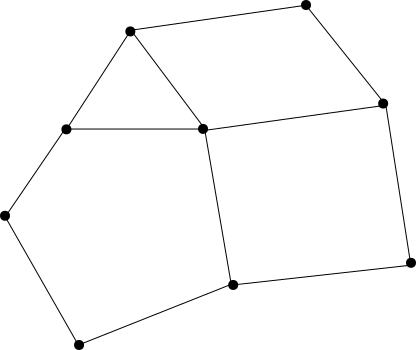
\includegraphics[width=0.3\textwidth]{MeshExample.pdf}
\end{figure}

\lstinputlisting[style=customc]{meshfacetraversal.js}


\end{frame}


\begin{frame}{Code Layout: Image Sources}

 \lstinputlisting[style=customc]{imagesources.js}       

\end{frame}

\begin{frame}{Reflections / Projections}


\uncover<2->{
\begin{itemize}
\item Plane: $(\vec{q}, \vec{n})$

\item Point: $\vec{p}$


\item Reflection: $ \vec{p} - 2( (\vec{p}-\vec{q})\cdot n) \vec{n}$
\end{itemize}
}


\end{frame}


\begin{frame}{Ray Intersect Plane}

\uncover<2->{\[ (\vec{p_0} + t \vec{v} - \vec{q}) \cdot \vec{n} = 0 \]}

\uncover<3->{

\[ t = \frac{ (\vec{q} - \vec{p_0}) \cdot n }{ \vec{v} \cdot \vec{n} } \]

}

\end{frame}


\begin{frame}{Point Inside Convex Polygon: Area Test}

\begin{figure}[t]
\centering
\includegraphics[width=0.8\textwidth]{PointInsidePolygon.pdf}
\end{figure}


\end{frame}

\begin{frame}{Convex Polygon Area?}

\begin{figure}[t]
\centering
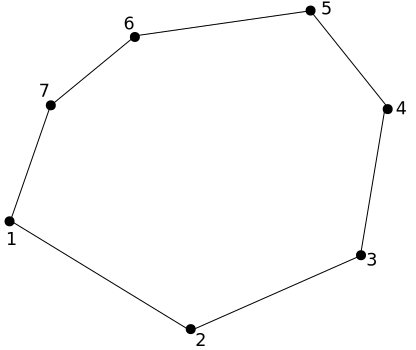
\includegraphics[width=0.8\textwidth]{PointInsidePolygonEmpty.pdf}
\end{figure}

\end{frame}


\begin{frame}{Convex Polygon Area: Triangle Fan}

\begin{figure}[t]
\centering
\includegraphics[width=0.8\textwidth]{TriangleFan.pdf}
\end{figure}


\end{frame}


\begin{frame}{Extra Stuff: Binaural Sound}

\begin{figure}[t]
\centering
\includegraphics[width=0.6\textwidth]{BinauralSound.png}
\end{figure}


\end{frame}

\begin{frame}{Extra Stuff: Transmission}

\begin{figure}[t]
\centering
\includegraphics[width=0.44\textwidth]{ImageSources2MultiDrawn4_Transmission.pdf}
\end{figure}

\[(r|t)*\]

\end{frame}



\begin{frame}{Extra Stuff: Transmission (Raffle Point)}

Regular expressions \uncover<2->{$(r|t)*$}

\begin{figure}[t]
\centering
\includegraphics[width=0.35\textwidth]{ImageSources2MultiDrawn4_Transmission.pdf}
\end{figure}



\end{frame}

\begin{frame}{Extra Stuff: Frequency dependent transmission}

\begin{figure}[t]
\centering
\includegraphics[width=0.8\textwidth]{outsidecar.png}
\end{figure}


\end{frame}


\begin{frame}{Extra Stuff: Bounding Box Speedup}

\begin{figure}[t]
\centering
\includegraphics[width=0.8\textwidth]{SceneGraphBBox.pdf}
\end{figure}


\end{frame}


\begin{frame}{Table of Contents}
\begin{itemize}[label=$\vartriangleright$]
	\item Assignment Concepts Review
\end{itemize}
\begin{itemize}[label=$\blacktriangleright$]
	\item PCA New Convention
\end{itemize}
\begin{itemize}[label=$\vartriangleright$]
	\item Procrustes Distance
\end{itemize}

\end{frame}

\begin{frame}{PCA New Convention}

Organize point cloud into $d \times N$ matrix, each point {\em along a column}

\[ X = \left[ \begin{array}{cccc} | & | & \hdots & | \\ \vec{v_1} & \vec{v_2} & \vdots & \vec{v_N} \\ | & | & \hdots & | \end{array} \right] \]

Choose a unit column vector direction $u \in \mathbb{R}^{d \times 1}$

Then 

\[ d = u^TX \]

gives projections onto $u$

\uncover<2->{
\begin{itemize}[label=$\vartriangleright$]
\item More consistent with what we've done; points in columns
\end{itemize}
}

\end{frame}

\begin{frame}{PCA New Convention}

\[ d = u^TX \]

\uncover<2->{
\begin{itemize}[label=$\vartriangleright$]
\item How to express the sum of the squares of the dot products?
\end{itemize}
}

\uncover<3->{
\[ dd^T \]
}

\uncover<4->{
\[ dd^T = (u^TX)(u^TX)^T = u^TXX^Tu \]
Want to find $u$ that maximizes the above quadratic form
}

\end{frame}

\begin{frame}{PCA New Convention}
Use eigenvectors of $A = XX^T$ to find principal directions maximizing $u^TAu$

\[\lambda_1 = 422 \]
\begin{figure}[t]
\centering
\includegraphics[width=0.7\textwidth]{2DPCADirMax.pdf}
\end{figure}


\end{frame}

\begin{frame}{PCA New Convention}
Use eigenvectors of $A = XX^T$ to find principal directions maximizing $u^TAu$

\[\lambda_2 = 21.6 \]
\begin{figure}[t]
\centering
\includegraphics[width=0.7\textwidth]{2DPCADirMin.pdf}
\end{figure}


\end{frame}





\begin{frame}{Table of Contents}
\begin{itemize}[label=$\vartriangleright$]
	\item Assignment Concepts Review
\end{itemize}
\begin{itemize}[label=$\vartriangleright$]
	\item PCA New Convention
\end{itemize}
\begin{itemize}[label=$\blacktriangleright$]
	\item Procrustes Distance
\end{itemize}

\end{frame}


\begin{frame}{Procrustes Distance}

\begin{figure}[t]
	\centering
    \includegraphics[width=0.6\textwidth]{procrustes.png}
\end{figure}

\url{http://www.procrustes.nl/gif/illustr.gif}

\end{frame}

\begin{frame}{Procrustes Alignment}

\begin{figure}[t]
	\centering
    \includegraphics[width=\textwidth]{ProcrustesEx1.png}
\end{figure}

\end{frame}


\begin{frame}{Procrustes Distance}

Given two point clouds $\{\vec{x_i}\}_{i=1}^N$ and $\{\vec{y_i}\}_{i=1}^N$

where $x_i$ and $y_i$ are in correspondence

Seek to minimize

\[ \sum_{i=1}^N ||R(\vec{x_i} + \vec{t}) - \vec{y_i}||_2^2 \]

over all orthogonal matrices $R$ and translation vectors $t$.  $||.||^2$ is squared distance

\end{frame}



\end{document}

